\section{AD Wandler \hartl{475}}

\subsection{Parallelverfahren und Kaskadenumsetzer}
\begin{longtable}{|p{12cm}|c|}
\hline
  {\textbf{Parallelumsetzer} \hartl{478}\newline
  \begin{itemize}
    \item sehr schnell
    \item $2^n$ Widerstände
    \item $2^N$ Komparatoren
  \end{itemize}
  \begin{align*}
    Anz_{Vergleiche}=2^N-1
  \end{align*}}
  &
  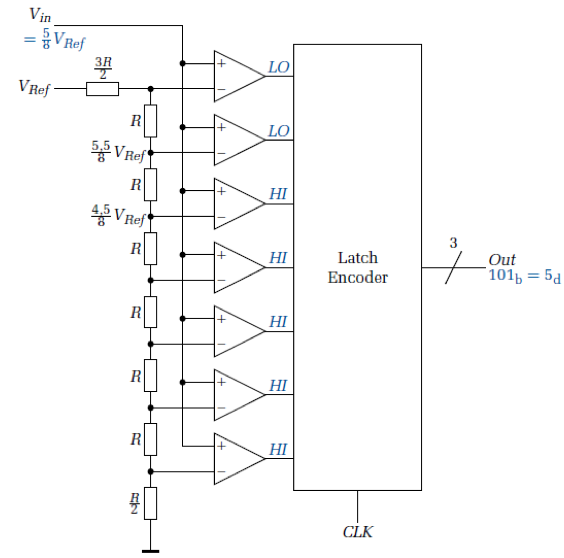
\includegraphics[width=6cm, valign=t]{pictures/parallelADC}\\ 
\hline

  {\textbf{Kaskadenumsetzer}\hartl{479}\newline 
  Eine 10-bit-Auflösung beim Parallelverfahren würde 1024 Komperatoren
  benötigen.$\Rightarrow$Komplexitätsreduktion \newline
  Mit erstem $N_{1}$-bit ADU wird der Grobbereich festgelegt (höherwertige
  Bits).
  Diese Zahl wird in eine analoge Spannung durch einen $N_{1}$-bit DAU zurück
  umgesetzt und diese Spannung von der Eingangsspannung subtrahiert. Diese
  Differenz wird von einem weiteren $N_{1}$-bit-ADU umgesetzt, um die
  niederwertigen Bits zu ergeben. Skaliert man die Differenzspannung mit dem
  Faktor 32, hat man den gleichen Spannungsbereich, kann also zwei identische
  ADC benutzen.
  }
  &
  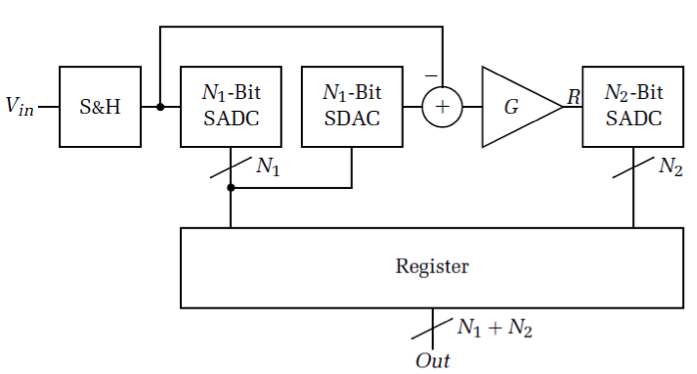
\includegraphics[width=6cm, valign=t]{pictures/kaskaden}\\ 
\hline

  {\textbf{Pipelined ADC} \hartl{483} \newline
  \begin{itemize}
    \item fast gleiche hohe Umsetzrate wie Parallelumsetzer
    \item gleicher schaltungstechnischer Aufwand wie beim Kaskadennumsetzer
    \item wird heute für schnelle ADC's verwendet
  \end{itemize}
  }
  &
  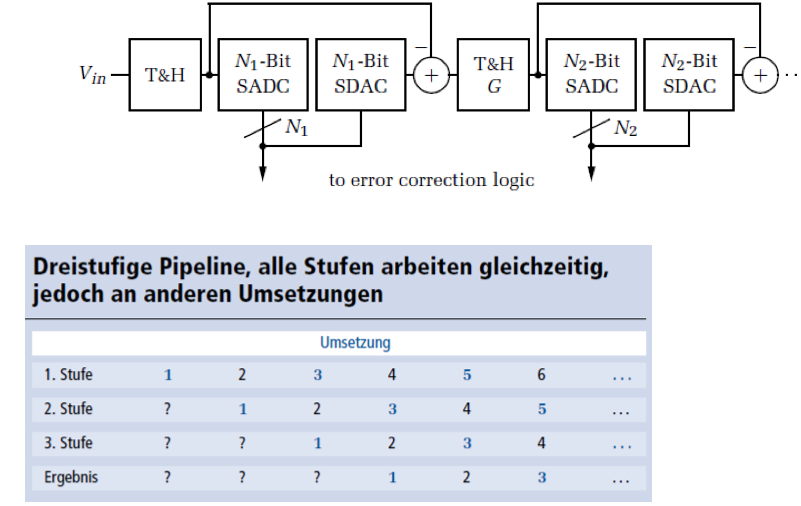
\includegraphics[width=6cm, valign=t]{pictures/pipelined}\\ 
\hline
\end{longtable}

\newpage
\subsection{Wägeverfahren ( sukzessive Approximation) \hartl{485}}
\begin{longtable}{|p{12cm}|c|}
\hline
  \multirow{2}{12cm}{\textbf{Prinzip} \hartl{485}
  \begin{itemize}
    \item Abtastung der Eingangsspannung $V_{in}$mit einer
        S\&H-Schaltung( Vergleichsspannung liegt so während der gesamten
      Umsetzung an)
    \item Vergleich starte in der Mitte der Eingangsspannung $\frac{V_{Ref}}{2}$
  \end{itemize}
  }
  &
  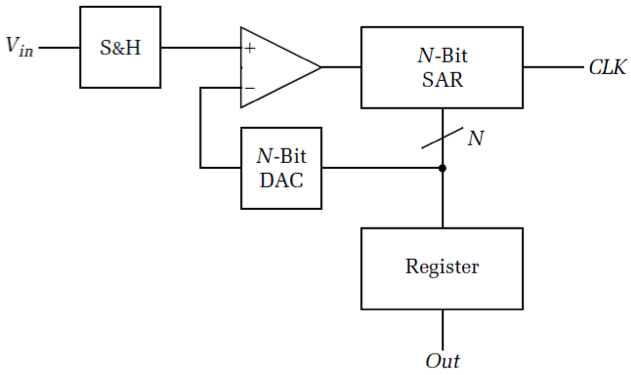
\includegraphics[width=6cm, valign=t]{pictures/waegeverfahren}\\
     &
  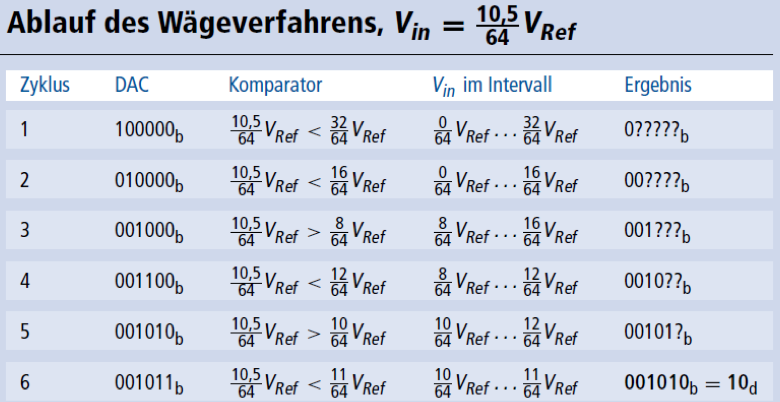
\includegraphics[width=6cm, valign=t]{pictures/waegeverfahrentabelle}\\
\hline

  {\textbf{Wägeverfahren mit SC-Prinzip} \hartl{488}\newline
  \begin{itemize}
    \item häufig eingesetze Implementierung
    \item mit geschalteten Kapazitäten ist es möglich Halte-Glied und DAc in
    einer Schaltung zu realisieren
  \end{itemize}
  \begin{enumerate}
    \item Schalter $S_{2},S_{1},S_{0},S_{A}$ verbunden mit $V_{in}$ und
      $S_{C}$mit GND$\to$ alle Kapazitäten werden auf $V_{in}$aufgeladen
    \item öffnen der Schalter $S_{C}und S_{A}$ und bleiben in dieser Stellung
    \item $S_{2}$ auf $V_{Ref}$ und $S_{1},S_{0}$auf GND $\to$
      $V_{x}=-V_{in}+0,5V_{Ref}$
    \item Ergebnis von SAR ausgewertet $\to$ $S_{2}$bleibt oder wechselt auf GND
    \item Fortzetung mit den folgenden Schaltern
  \end{enumerate}
  }
  &
  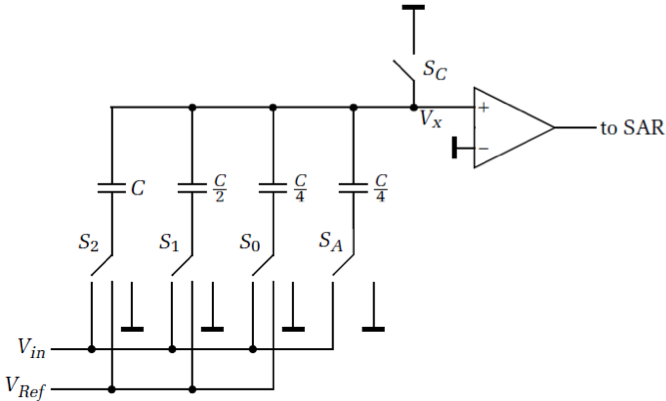
\includegraphics[width=6cm, valign=t]{pictures/waegeverfahrenSC}\\
\hline

  {\textbf{Iterative ADC} \newline
  \begin{enumerate}
    \item Im S/H wird die Eingangsspannung geschpeichert (Schalter Sin)
    \item Schalter Sin wird danach auf den Multiplizierer-Ausgang geschaltet
    \item X(Laufvariable) wird auf n-1 gesetzt
    \item Der Jomparator wird ausgewertet\newline
      Dout=1: Bx=1, Switch S=1 (d.h. im Subtrahierer wird Vrefh von Vc
      subtrahiert)\newline
      Dout=0: Bx=0, Switch S=0 (d.h. im Subtrahierer wird 0 von Vc
      subtrahiert)
    \item Der Subtrahierer generiert sein Ausgangssignal
    \item Der Multiplizierer generiert sein Ausgangssignal
    \item Im S/H wird die Feedback-Spannung gespeichert (Schalter Sin)
    \item X wird um 1 reduziert
    \item Gehe zu Schritt 4, wenn $X\geq0$
  \end{enumerate}
  }
  &
  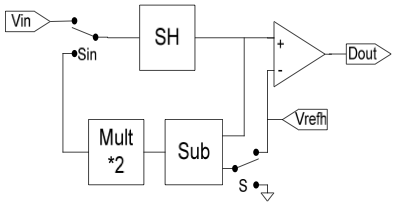
\includegraphics[width=6cm, valign=t]{pictures/iterativeADC}\\
\hline
\end{longtable}



\subsection{Zählverfahren \hartl{490}} 
Ist für kontinuierliche Auswertungen des Eingangssignal
\subsubsection{Single Slope}

\begin{tabular}{ccp{4cm}}
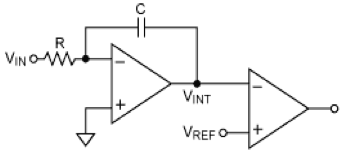
\includegraphics[width=6cm, valign=t]{pictures/singleSlope1}
&
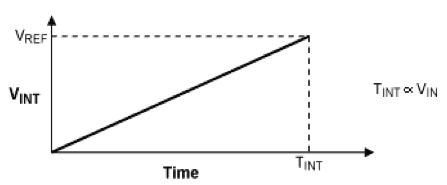
\includegraphics[width=6cm, valign=t]{pictures/singleSlope2}
&
  {\begin{align*}
    T_{int}=\frac{V_{Ref}*R*C}{V_{in}}
  \end{align*}}
\\ 
\end{tabular}

\subsubsection{Dual Slope \hartl{492}}
\begin{tabular}{cp{12cm}}
 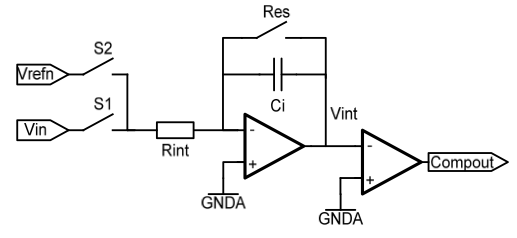
\includegraphics[width=6cm, valign=t]{pictures/dualSlope11}
 & 
 {Für $0<t<T_{int}$
 \begin{align*}
      V(t)&=
      \int\limits_0^{t}\frac{-1}{R_{int}
      \cdot C_{i}}(V_{in}-V_{GNDA})dt+V_{GNDA}\\
      V_{int}(V_{in})&=\frac{-1}{R_{int}
      \cdot C_{i}}(V_{in}-V_{GNDA})T_{int}+V_{GNDA}\\
      V_{intmax}&=V_{int}(V_{in}=0)\\
                &=\frac{-1}{R_{int}
      \cdot C_{i}}(-V_{GNDA})T_{int}+V_{GNDA}
 \end{align*}} \\
 
 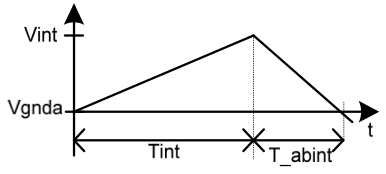
\includegraphics[width=6cm, valign=t]{pictures/dualSlope12}
 &  
 {Für $T_{int}<t<T$
 \begin{align*}
  V(t)&=V_{int}-\frac{1}{R_{int}\cdot C_{i}}\cdot
  (V_{refn}-V_{GNDA}) \cdot t\\
   T_{abint}&=\frac{(V_{GNDA}-V_{in}) \cdot T_{int}}{V_{refn}-V_{GNDA}}
 \end{align*}}\\
 
 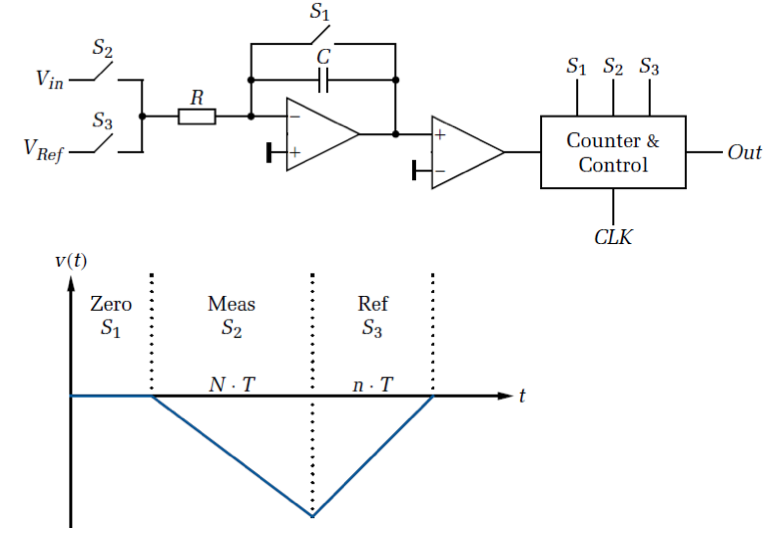
\includegraphics[width=6cm, valign=t]{pictures/dualSlope2}
 &  
 {Für $V_{GNDA}=0$:
  \begin{align*}
    \int^{NT}_{0}V_{in}dt&=NTV_{in}\\
      NTV_{in}-\int^{nT}_{0}V_{Ref}dt&=NTV_{in}-nTV_{Ref}=0\\
      n&=\frac{V_{in}}{V_{Ref}}N\\
  \end{align*}}\\
  
  
  \begin{tabular}{ll}
      N:&Taktzyklen\\
      T:&Periodendauer\\
      n:&Zählerstand\\
      $V_{off}$:&Offsetspannung\\
  \end{tabular}
  &
  
  \begin{tabular}{ll}
      $T_{int}$:&Integrationszeit\\
      $T_{abint}$:& "`Messzeit"\\
      $V_{int}$:&Spannung am $V_{opOut}$ nach der Zeit $T_{int}$\\
      $V_{intmax}:$&maximal mögliche Spannung am $V_{opOut}$\\
  \end{tabular}
\end{tabular}
\newpage

\subsubsection{Spannungs- Frequenz- Umsetzer \hartl{495}}
\begin{tabular}{cp{12cm}}
  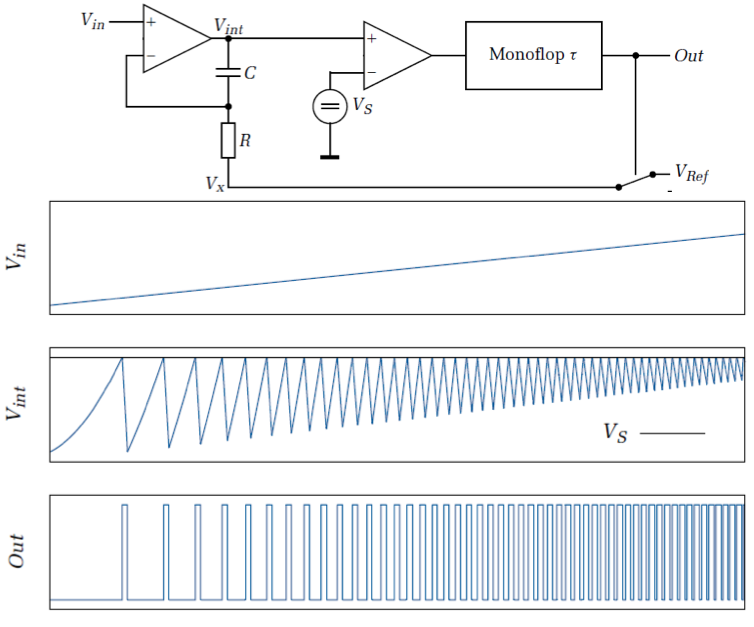
\includegraphics[width=6cm, valign=t]{pictures/sfu}
  &
    {\begin{align*}
      V_{int}(t)=V_{in}+\frac{1}{RC}\int(V_{in}-V_{x})dt
    \end{align*}
    Vorteil: Immer am Eingangssignal\newline
    Nachteil: Kein echter ADC}\\
\end{tabular}


\subsubsection{Ladungs-Ausgleichs-Integrator \hartl{497}}
\begin{tabular}{cp{12cm}}
  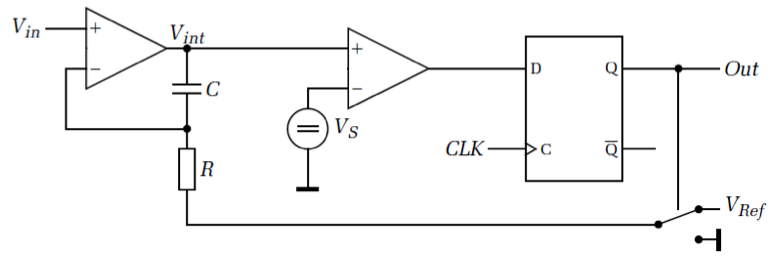
\includegraphics[width=6cm, valign=t]{pictures/lsg1}
  &
  \multirow{2}{12cm}{
    \begin{itemize}
      \item Gleichgewichtsbedingung\\
        \begin{equation}
          V_{in}-\frac{n}{N}V_{Ref}=0\Rightarrow n=\frac{V_{in}}{V_{Ref}}N
        \end{equation}
      \item Flipflop statt Monoflop
    \end{itemize}}\\ 
  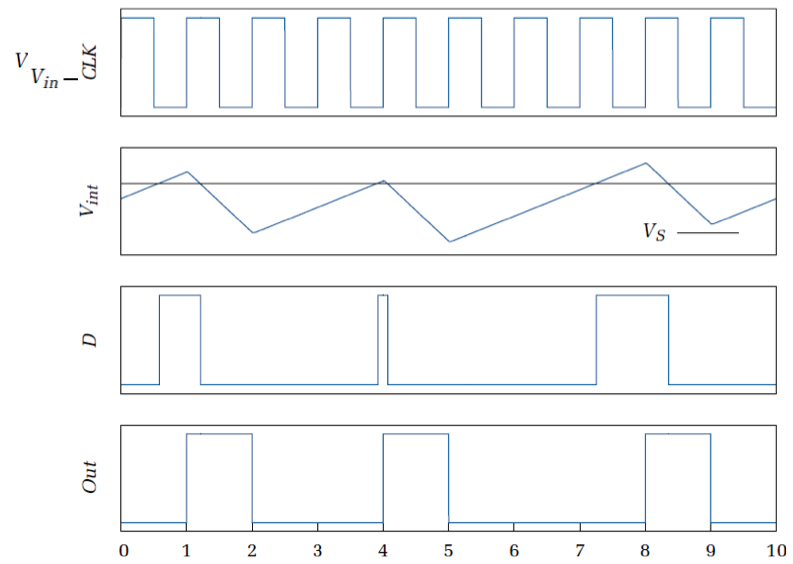
\includegraphics[width=6cm, valign=t]{pictures/lsg2}
  & \\
\end{tabular}


\subsubsection{Sigma-Delta Wandler \hartl{500}}
\begin{tabular}{cp{12cm}}
  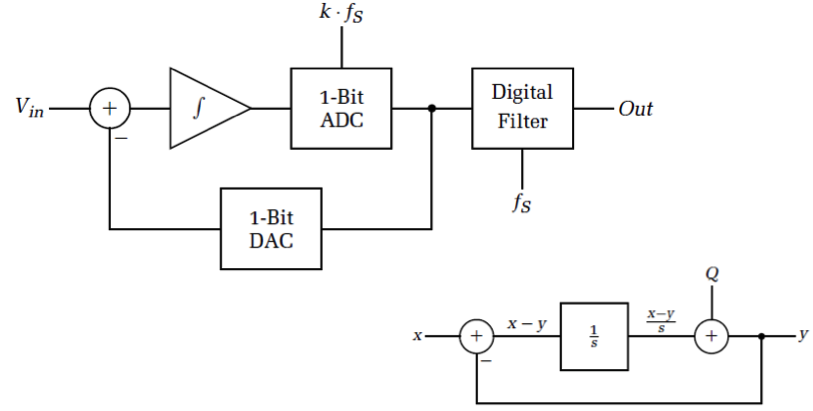
\includegraphics[width=6cm, valign=t]{pictures/deltaSigma1}
  &
  {\begin{itemize}
      \item Ersatzschaltung für Frequenzbereich
      \item Tiefpass für Signal
      \item Hochpass für Q
    \end{itemize}
    \begin{align*}
      y=\frac{x-y}{s}+Q\Rightarrow y=x\frac{1}{1+s}+Q\frac{s}{1+s}
    \end{align*}
  }\\
\end{tabular}


\subsubsection{Sigma-Delta Wandler 2. Ordnung \hartl{502}}
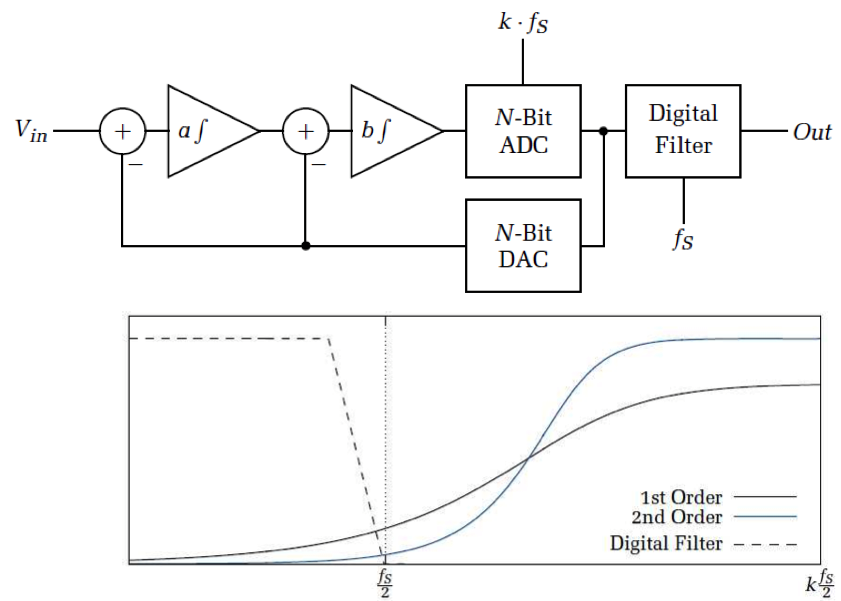
\includegraphics[width=6cm, height =4cm]{pictures/deltaSigma2}



\subsection{Kennwerte von ADC's}
\begin{figure}[!htbp]
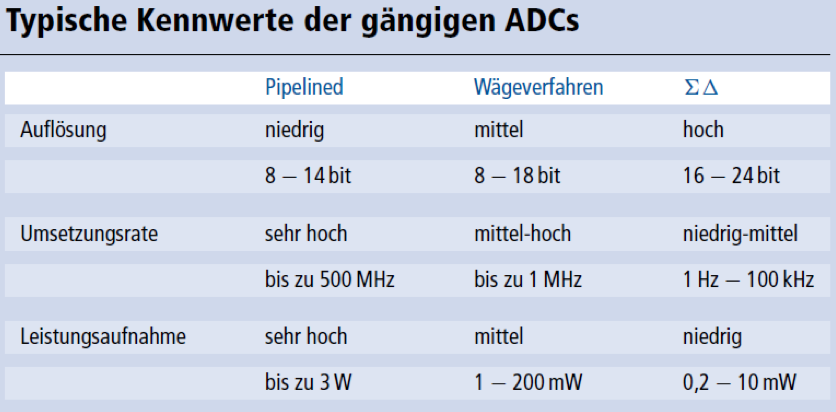
\includegraphics[scale=0.4]{pictures/kennwerteADC}
\end{figure}

